\chapter{Perancangan}
\label{chap:design}

Berdasarkan analisa dari bab 3, pada bab ini akan dibahas mengenai perancangan diagram kelas, dan perancangan antarmuka dari
program.

\section{Perancangan Diagram Kelas}
\begin{figure}[H]
	\centering
	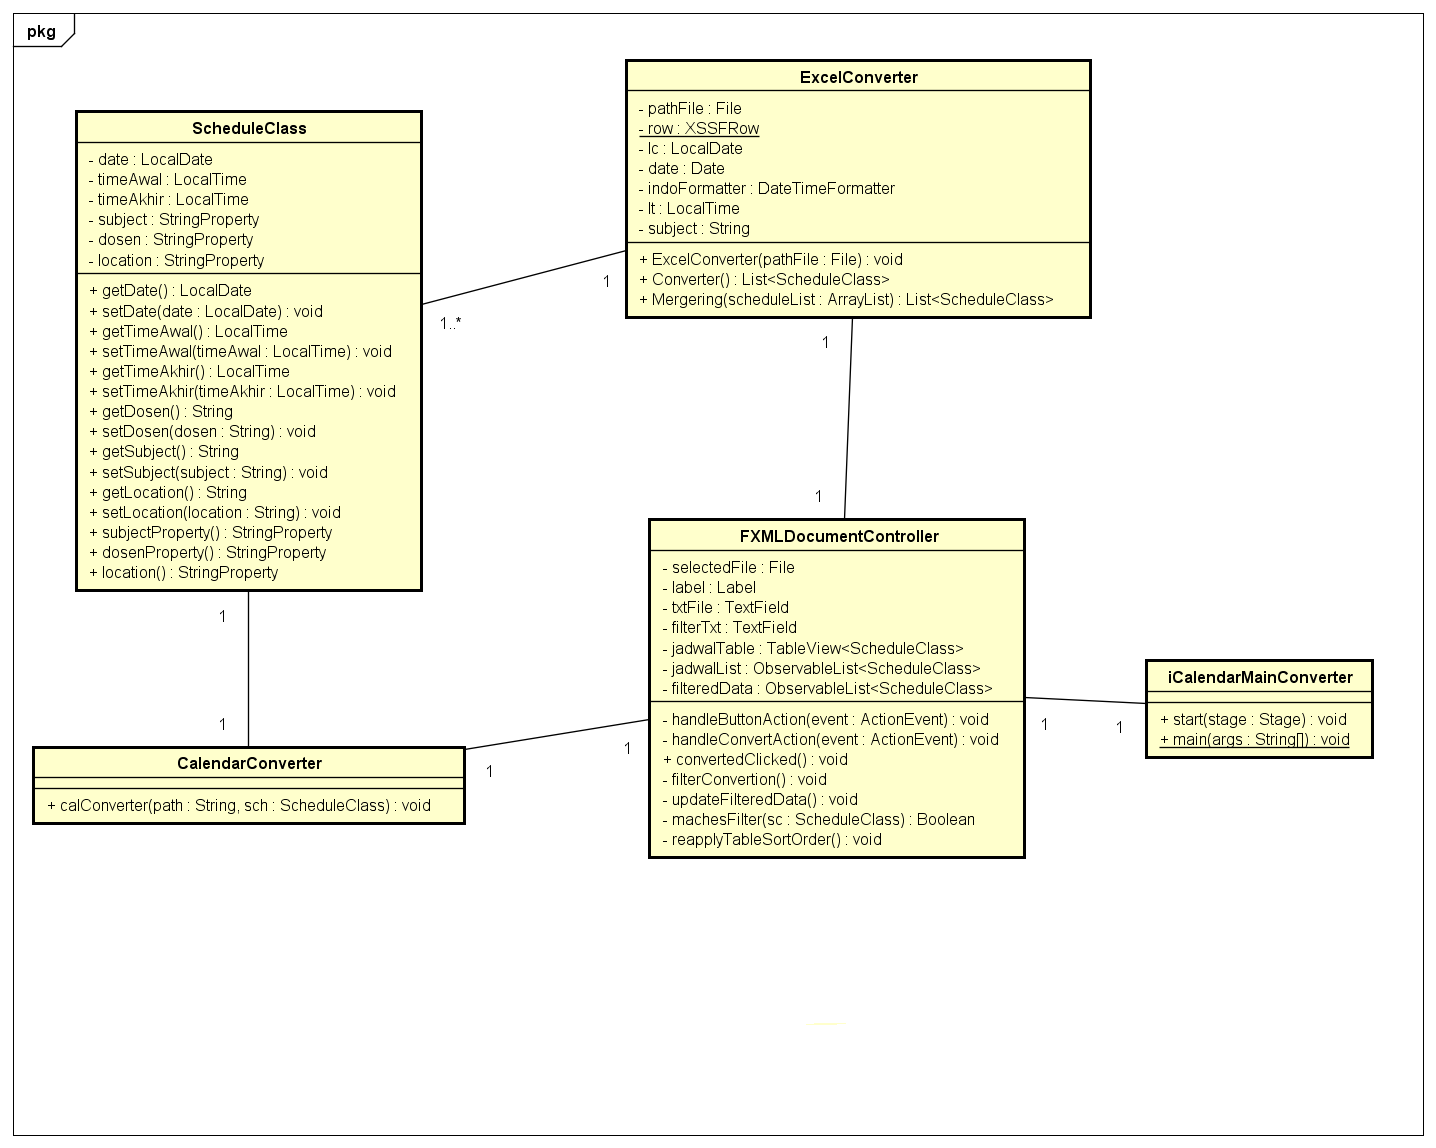
\includegraphics[scale=0.4]{Gambar/kelas-diagram}
	\caption{Gambar Kelas Diagram}
	\label{fig:pemodelan-kelas}
\end{figure}

Berikut ini rincian kelas pada diagram kelas yang tercantum dalam tabel-tabel dibawah ini :

\begin{table}[H]
	\centering
		\caption{Tabel Kelas \textit{ScheduleClass}}
		\label{tab:schedule_class}
		\begin{tabular}{ | c | c | c |}
			\hline
				\multicolumn{3}{|c|}{Atribut} \\ \hline 
				Nama atribut & Tipe Data  & Fungsi \\ \hline
				date & LocalDate & Atribut tanggal\\ \hline
				timeAwal & LocalTime & Atribut jam ujian dimulai\\ \hline
				timeAkhir & LocalTime & Atribut jam ujian berakhir\\ \hline
				subject & StringProperty & Atribut mata kuliah\\ \hline
				dosen & StringProperty & Atribut nama dosen\\ \hline
				location & StringProperty & Atribut lokasi ujian\\ \hline
				\multicolumn{2}{|c|}{Method} & Fungsi \\ \hline
				\multicolumn{2}{|l|}{getDate()} & Mendapatkan tanggal\\ \hline
				\multicolumn{2}{|l|}{setDate(date: LocalDate)} & Set tanggal \\ \hline
				\multicolumn{2}{|l|}{getTimeAwal()} & Mendapatkan jam awal ujian \\ \hline
				\multicolumn{2}{|l|}{setTimeAwal(timeAwal: LocalTime)} & Set jam awal ujian\\ \hline
				\multicolumn{2}{|l|}{getTimeAkhir()} & Mendapatkan jam akhir ujian\\ \hline
				\multicolumn{2}{|l|}{setTimeAkhir(timeAkhir: LocalTime)} & Set jam akhir ujian\\ \hline
				\multicolumn{2}{|l|}{getDosen()} & Mendapatkan nama dosen\\ \hline
				\multicolumn{2}{|l|}{setDosen(dosen: String)} & Set nama dosen\\ \hline
				\multicolumn{2}{|l|}{getSubject()} & Mendapatkan nama mata kuliah\\ \hline
				\multicolumn{2}{|l|}{setSubject(subject: String)}& Set mata kuliah \\ \hline
				\multicolumn{2}{|l|}{getLocation()} & Mendapatkan lokasi ujian\\ \hline
				\multicolumn{2}{|l|}{setLocation(location: String)} & Set lokasi ujian\\ \hline
				\multicolumn{2}{|l|}{subjectProperty()} & Mendapatkan properti mata kuliah\\ \hline
				\multicolumn{2}{|l|}{dosenProperty()} & Mendapatkan properti dosen\\ \hline
				\multicolumn{2}{|l|}{location()} & Mendapatkan properti lokasi\\ \hline
		\end{tabular}
\end{table}

\begin{table}[H]
	\centering
		\caption{Tabel Kelas \textit{ExcelConverter}}
		\label{tab:excel_converter}
		\begin{tabular}{ | c | c | p{4cm} |}
			\hline
				\multicolumn{3}{|c|}{Atribut} \\ \hline 
				Nama atribut & Tipe Data  & Fungsi \\ \hline
				pathFile & File & Atribut path file excel mengawas\\ \hline
				row & XSSFRow & Atribut baris dari Excel\\ \hline
				lc & LocalDate & Atribut tanggal ujian\\ \hline
				indoFormater & DateTimeFormatter & Atribut konversi ke timezone jakarta\\ \hline
				lt & LocalTime & Atribut jam ujian\\ \hline
				subject & String & Atribut matakuliah\\ \hline
				\multicolumn{2}{|c|}{Method} & Fungsi \\ \hline
				\multicolumn{2}{|c|}{ExcelConverter(path: File)} & Konstruktor untuk mendapatkan path file dari excel mengawas ujian\\ \hline
				\multicolumn{2}{|c|}{Converter()} & Konversi excel menjadi list scheduleClass \\ \hline
				\multicolumn{2}{|c|}{Mergering(scheduleList: ArrayList)} & Mengabungkan entri mengawas dosen  duplikat menjadi satu mata kuliah \\ \hline
		\end{tabular}
\end{table}

\begin{table}[H]
	\centering
		\caption{Tabel Kelas \textit{CalendarConverter}}
		\label{tab:excel_converter}
		\begin{tabular}{ | c | c | p{4cm} |}
			\hline
				\multicolumn{2}{|c|}{Method} & Fungsi \\ \hline
				\multicolumn{2}{|c|}{calConverter(path: String, sch: ScheduleClass)} & Mengkonversi scheduleClass yang dipilih kedalam iCal dan menyimpannya pada path yang ditentukan\\ \hline
		\end{tabular}
\end{table}

\begin{table}[H]
	\centering
		\caption{Tabel Kelas \textit{FXMLDocumentController}}
		\label{tab:FXMLDocumentController}
		\begin{tabular}{ | c | c | p{4cm} |}
			\hline
				\multicolumn{3}{|c|}{Atribut} \\ \hline 
				Nama atribut & Tipe Data  & Fungsi \\ \hline
				selectedFile & File & Atribut file yang dipilih user\\ \hline
				label & Label & Atribut label\\ \hline
				txtFile & TextField & Atribut menampilkan path file yang dipilih\\ \hline
				filterTxt & TextField & Atribut untuk menampilkan filter teks\\ \hline
				jadwalTable & TableView<ScheduleClass> & Atribut menampilkan tabel jadwal\\ \hline
				jadwalList & ObservableList<ScheduleClass> & Atribut untuk menyimpan jadwal\\ \hline
				filteredData & ObservableList<ScheduleClass> & Atribut untuk menyimpan data yang telah di filter\\ \hline
				\multicolumn{2}{|c|}{Method} & Fungsi \\ \hline
				\multicolumn{2}{|c|}{handleButtonAction(event: ActionEvent)} & Method untuk melakukan browse dan menyimpan file excel\\ \hline
				\multicolumn{2}{|c|}{handleConvertAction(event: ActionEvent)} & Method untuk membaca file excel \\ \hline
				\multicolumn{2}{|c|}{convertedClicked()} & Method untuk konversi \textit{selected item} menjadi iCal  \\ \hline
				\multicolumn{2}{|c|}{filterConvertion()} & Method untuk menerima masukan filter dari user \\ \hline
				\multicolumn{2}{|c|}{updateFilteredData()} & Menginisiasi list filteredData \\ \hline
				\multicolumn{2}{|c|}{matchesFilter(sc: ScheduleClass)} & Mencocokan nama dosen sesuai yang di inginkan user \\ \hline
				\multicolumn{2}{|c|}{reapplyTableSortOrder()} & Mengatur urutan tabel setelah di filter \\ \hline
		\end{tabular}
\end{table}

\begin{table}[H]
	\centering
		\caption{Tabel Kelas \textit{iCalendarMainConverter}}
		\label{tab:iCalendarMainConverter}
		\begin{tabular}{ | c | c | p{4cm} |}
			\hline
				\multicolumn{2}{|c|}{Method} & Fungsi \\ \hline
				\multicolumn{2}{|c|}{start(stage: Stage)} & Menampilkan window\\ \hline
			\multicolumn{2}{|c|}{main(args: String[])} & Mengeksekusi program\\ \hline
		\end{tabular}
\end{table}

\section{Perancangan Antarmuka}
Setelah melalui serangkaian anlisa dan perancangan diagram kelas bapa sub bab ini akan dijelaskan mengenai gambaran bentuk program mengawas ujian tersebut.

\begin{enumerate}
	\item Halaman awal program 
		\begin{figure}[H]
		\centering
		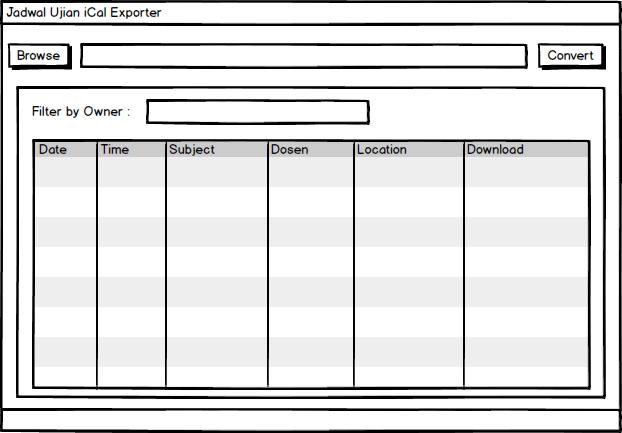
\includegraphics[scale=0.5]{Gambar/antarmuka}
		\caption{Tampilan awal Program}
		\label{fig:tampilan_awal}
		\end{figure}
	\item Halaman untuk melakukan \textit{Browse} file excel
		\begin{figure}[H]
		\centering
		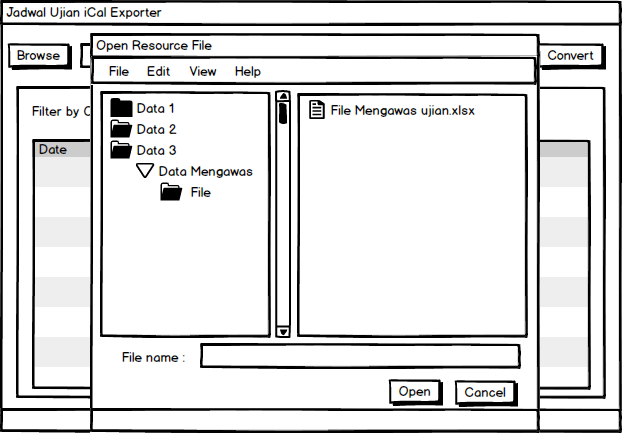
\includegraphics[scale=0.5]{Gambar/antarmuka3}
		\caption{Tampilan \textit{Browse} file excel}
		\label{fig:browse}
		\end{figure}
	\item Halaman setelah excel dibaca
		\begin{figure}[H]
		\centering
		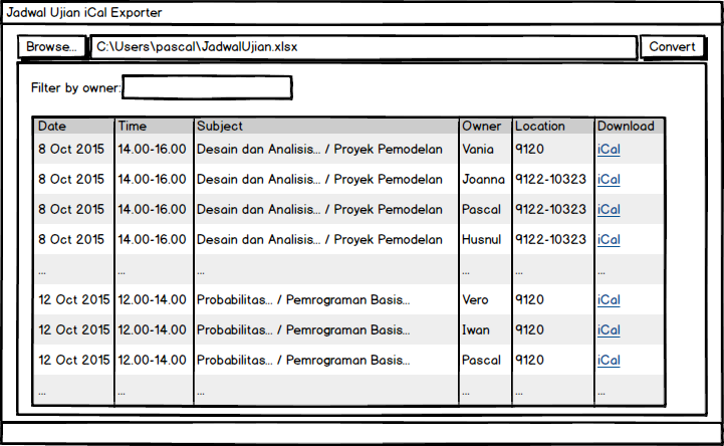
\includegraphics[scale=0.5]{Gambar/antarmuka2}
		\caption{Tampilan setelah excel dibaca}
		\label{fig:excel_dibaca}
		\end{figure}
	\item Halaman untuk menyimpan iCal
		\begin{figure}[H]
		\centering
		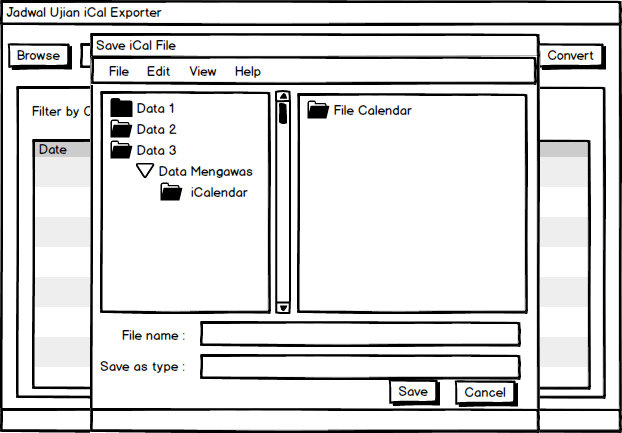
\includegraphics[scale=0.5]{Gambar/antarmuka4}
		\caption{Tampilan untuk menyimpan iCal}
		\label{fig:jadwalpng}
		\end{figure}
\end{enumerate}

\section{Rancangan \textit{Method-Method} Utama}
Berikut ini adalah rancangan \textit{method} utama program jadwal mengawas ujian yang akan dibangun perangkat lunaknya :
\begin{enumerate}
	\item Converter() \\
	\begin{tabular}{l c p{9cm}}
		Input & : & - \\ 
		Output & : & List<ScheduleClass> \\ 
		Deskripsi & : & Method ini membaca excel yang di input oleh user dan mengkonversikannya kedalam bentuk list\\
		Algoritma & : & \begin{enumerate}
			\item Ambil path file yang telah di input oleh user
			\item Cari kolom No. pada file excel dan jadikan acuan bahwa program akan membaca setelah dari index kolom tersebut
			\item Baca baris per baris namun cek terlebih dahulu apakah di kolom No. baris tersebut masih berupa nomer, apabila tidak maka berhenti membaca karena baris yang berisi jadwal sudah terbaca semua
			\item Cek apakah baris mengandung kata \textit{LIBUR} bila iya maka lewati saja
			\item Pisahkan hari dan tanggal lalu konversi menjadi localDate. 
			\item Pisahkan jam menjadi jamAwal dan jamAkhir, lalu konversi menjadi localTime.
			\item jika menemukan kata \textit{Shift} atau \textit{Lab} maka lokasi ujian adalah Lab
			\item Masukan semua kedalam sebuah arrayList<ScheduleClass>
		\end{enumerate}
		\end{tabular}	
	
	\item Mergering()\\
	\begin{tabular}{l c p{9cm}}
		Input & : & List<ScheduleClass> \\ 
		Output & : & List<ScheduleClass> \\ 
		Deskripsi & : & Method ini mengatasi duplikat \textit{entry} dari dosen yang mempunyai dua jadwal mengawas pada hari yang sama\\
		Algoritma & : & 
			\begin{enumerate}
				\item Cari subject/mata kuliah yang tidak memiliki dosen pada arrayList yang telah di proses oleh \textit{method} Convert() karena bila program membaca kolom merger maka hanya kolom pertama saja yang dibaca sehingga kolom keduanya kosong.
				\item Masukan baris yang tidak memiliki dosen kedalam arrayList baru
				\item Hapus baris yang tidak memiliki dosen pada arrayList master
				\item Cocokan waktu dan tanggal ujian arrayList master dengan temp, bila sama maka tambahkan matakuliah/subject pada arrayList master
			\end{enumerate}
		\end{tabular}	
	
	\item calConverter()\\
	\begin{tabular}{l c p{9cm}}
		Input & : & sch: ScheduleClass , path: String\\ 
		Output & : & void \\ 
		Deskripsi & : & Method ini mengkonversi ScheduleClass menjadi iCal\\
		Algoritma & : & 
			\begin{enumerate}
				\item Inisiasi variable timezone Indonesia
				\item Konversi tanggal, bulan, dan tahun kedalam GregorianCalender
				\item Masukan event berdasarkan subject/mata kuliah , lokasi, dan dosen yang mengawas.
				\item Inisiasi kalender dan masukan variable tanggal dan event yang telah dibuat sebelumnya kedalam variable kalender tersebut
				\item Simpan pada path yang telah di pilih oleh user
			\end{enumerate}
		\end{tabular}	
		
	\item filterConvertion()\\
	\begin{tabular}{l c p{9cm}}
		Input & : & void\\ 
		Output & : & void \\ 
		Deskripsi & : & Method ini menjalankan filter data dosen sesuai input user\\
		Algoritma & : & 
			\begin{enumerate}
				\item Inisiasi tabel dengan list yang sudah di filter
				\item Masukan nilai yang sama kedalam list filter jika dosen yang dicari sesuai dengan input user.
				\item Atur kembali urutan tabel pada perangkat lunak
			\end{enumerate}
		\end{tabular}	
\end{enumerate}
